% inspired from: https://github.com/SnipyJulmy/hesso-latextemplate-lab
\documentclass[11pt,a4paper,oneside]{report}
\usepackage[margin=2cm]{geometry}
\usepackage[utf8]{inputenc}
\usepackage[T1]{fontenc}
\usepackage[french]{babel}
\usepackage{minted}
\usepackage{titlesec}
\usepackage[pdftex]{graphicx} % graphics importing
\usepackage{titling} % can use \theauthor \thetitle
\usepackage{parskip} % remove first line indenting in a section
\usepackage{microtype} % typographic improvements
\usepackage[defaultlines=3,all]{nowidow}
\usepackage[toc,page]{appendix}
\usepackage{verbatim}
\usepackage{float}
\usepackage{enumerate}

% == Header and Footer
\usepackage{fancyhdr}

% style for all normal pages
\fancypagestyle{normal}{
\fancyhf{}
\setlength\headheight{14pt}
\lhead[]{Docker and Embedded systems}
\chead[]{}
\rhead{
\includegraphics[width=3cm]{img/mse_logo}}
\lfoot[]{}
\cfoot[]{\thepage}
\rfoot[]{}
\renewcommand{\headrulewidth}{0.4pt}% Default \headrulewidth is 0.4pt
\renewcommand{\footrulewidth}{0.4pt}% default is 0pt
}

% style for history
\fancypagestyle{historystyle}{
\setlength\headheight{14pt}
\lhead[]{Docker and Embedded systems}
\chead[]{}
\rhead{
\includegraphics[width=3cm]{img/mse_logo}}
\lfoot[]{}
\cfoot[]{}
\rfoot[]{}

\renewcommand{\headrulewidth}{0.4pt}% Default \headrulewidth is 0.4pt
\renewcommand{\footrulewidth}{0pt}
}

\usepackage[hyphens]{url} % line wrap urls
\usepackage{hyperref}

% == Version history
\usepackage{vhistory}


% == Code snippets
\newminted{bash}{xleftmargin=20pt, linenos=true, breaklines=true, frame=single, framesep=6pt, tabsize=2, fontfamily=courier, fontsize=\small}

% inline code
\newcommand{\code}[1]{\texttt{#1}}

% == Chapter titles
% Remove space before title
\titlespacing{\chapter}{0pt}{*-4}{*3}
% Remove "Chapter N" and use a sans-serif font
\titleformat{\chapter}{\normalfont\huge}{\thechapter.}{20pt}{\huge}
% Change chapter page style
\patchcmd{\chapter}{plain}{fancy}{}{}



% Metadata
\newcommand{\school}{Haute École d'ingénierie et d'architecture de Fribourg}
\newcommand{\oldreportname}{État de l’art à la mi-projet de semestre Docker and embedded systems - Ou comment ne pas cross compiler Docker sur ARM}

\title{Projet de semestre Docker and embedded systems}
\author{Gary \bsc{Marigliano}}

% aliases
\newcommand{\odroid}{ODROID-XU3 Lite }

\begin{document}

\begin{titlepage}
\begin{center}


\includegraphics[width=0.6\textwidth]{img/docker_logo}\\[1cm]

\begin{figure}[htbp]
\begin{minipage}[c]{.45\linewidth}
\begin{flushleft}

\includegraphics[width=7cm]{img/mse_logo}
\end{flushleft}
\end{minipage}
\hfill
\begin{minipage}[c]{.45\linewidth}
\begin{flushright}

\includegraphics[height=2cm]{img/logo_hes-so}
\end{flushright}
\end{minipage}
\end{figure}

% Title
\rule{\linewidth}{0.5mm} \\[0.4cm]
{ \huge \bfseries \thetitle \\[0.4cm] }
\rule{\linewidth}{0.5mm} \\[1.5cm]

% Author and supervisor
\noindent
\begin{minipage}{0.4\textwidth}
  \begin{flushleft} \large
    \emph{Auteur :}\\
    \theauthor
  \end{flushleft}
\end{minipage}%
\begin{minipage}{0.4\textwidth}
  \begin{flushright} \large
    \emph{Encadrant :} \\
    Jean-Roland \bsc{Schüler}
  \end{flushright}
\end{minipage}

\vfill

\noindent
\begin{minipage}{0.4\textwidth}
  \begin{flushleft} \large
    \emph{Contact :}\\
    gary.marigliano@master.hes-so.ch
  \end{flushleft}
\end{minipage}%
\begin{minipage}{0.4\textwidth}
  \begin{flushright} \large
    \emph{Mandant :} \\
    \school
  \end{flushright}
\end{minipage}

\vfill

% Bottom of the page
{\large Version 0.0.1 \\ \today}

\end{center}
\end{titlepage}

\pagestyle{historystyle}
\begin{versionhistory}  
  \vhEntry{0.0.1}{02.05.16}{\theauthor}{Création du document}
\end{versionhistory}


\chapter{Résumé du document}

TODO

\pagenumbering{gobble}
\tableofcontents
\pagenumbering{arabic}

\pagestyle{normal}

\chapter{Introduction}

\section{Contexte}\label{contexte}

Ce document est le rapport de fin de projet de semestre Docker and embedded systems. Un des buts de ce projet est de cross compiler Docker à partir de ses sources pour produire un binaire exécutable sur un \odroid (ARMv7). De plus, une partie concernant la sécurité de Docker est également traitée.

Lien: \url{https://github.com/krypty/docker_and_embedded_systems}

Ce projet de semestre s'inscrit dans une certaine continuité avec les projets de semestre et de bachelor de M. Loic Bassang \cite{TODO}. Plusieurs pistes intéressantes avaient en effet été mentionnées dans ces projets là notamment une partie concernant la sécurité et Docker. Ainsi, ce rapport fera parfois des parallèles avec ces documents.

Il est important de noter que la vitesse de développement de Docker est assez hallucinante. En effet, sur Github (\url{https://github.com/docker/docker}) les commits se succèdent à vitesse grand V. Entre chaque version de Docker qui sortent environ tous les mois, il est courant d'avoir plus de 3000 commits qui ont été \emph{pushés}. Tout ceci pour dire qu'à la lecture de ce document, il est quasiment sûr que certaines pistes explorées soient définitivement obsolètes ou au contraire deviennent la voie à suivre du à une mise à jour quelconque.


\section{Objectifs}

De manière plus précise, ce projet vise à maitriser les parties suivantes:

\begin{enumerate}
  \item Construction d'un système Linux capable de faire tourner Docker et son \emph{daemon} en utilisant Buildroot. Pour générer le dit système, on dispose d'un \emph{repository} Gitlab hébergé à la \school

  \item Cross compilation de Docker et de son \emph{daemon}, capable de faire tourner des containers
  
  \item Comprendre, analyser et évaluer l'aspect sécurité de Docker dans le cadre d'une utilisation avec une carte embarquée
\end{enumerate}

Les deux premiers points ont été traités dans un précédent rapport appelé "\oldreportname".

Ce document se concentre, dès lors, sur le dernier point ainsi que sur le déroulement global du projet.


\chapter{Présentation de Docker}

\textbf{Remarque : } Si le lecteur a déjà lu le rapport "\oldreportname", il ne lui est pas nécessaire de relire ce chapitre sachant qu'il s'agit du même contenu.

\newcommand{\bassangPrjSemestre}{Docker and Internet of Things (travail de semestre)}
\newcommand{\bassangPrjBachelor}{Docker and Internet of Things (travail de Bachelor)}
\section{Introduction}

Le but de ce chapitre est d'apporter un contexte au projet réalisé afin de comprendre ce qui est expliqué dans la suite de ce document. Si le lecteur souhaite connaître les tréfonds de Docker, il est recommandé de lire le rapport "\bassangPrjSemestre" de M. Loic Bassang \cite{bassang_semestre}. 

Docker est un outil qui permet d'empaqueter une application et ses dépendances dans un container léger, auto-suffisant, isolé et portable. En intégrant leur application dans un container, les développeurs s'assurent que celle-ci va tourner sur n'importe quel environnement GNU/Linux. Ainsi, le temps passé à configurer les différents environnements (développement, test et production typiquement) est réduit, voire même unifié\cite{shipping_container_linux_code}\cite{wikipedia_docker}\cite{what_is_docker}.

Les caractéristiques principales des containers Docker sont les suivantes :
\begin{itemize}
\item \textit{légers} : les containers partagent le même kernel et librairies que le système d'exploitation hôte permettant ainsi un démarrage rapide des containers et une utilisation mémoire contenue
\item \textit{isolés} : les containers sont isolés grâce à des mécanismes offerts par le kernel. Voir section \ref{pres-docker-isolation} pour plus de détails
\item \textit{éphémères et maintenables} : les containers sont conçus pour être créés et détruits régulièrement contrairement à un serveur ou une machine virtuelle pour lesquels un arrêt est souvent critique. Ils sont maintenables dans le sens où il est possible de revenir à une version précédente facilement et qu'il est aisé de déployer une nouvelle version
\end{itemize}

Les sections qui suivent abordent un peu plus en profondeur certains points clés de Docker qui ont été jugés importants.

\section{Containers vs machines virtuelles}
Suite à la lecture de la section précédente, il serait normal de se dire que ces containers partagent certaines caractéristiques avec les machines virtuelles.

Voici les différences majeures qu'il existe entre les containers et les machines virtuelles\cite{what_is_docker}.

\begin{figure}[hbtp]
\centering
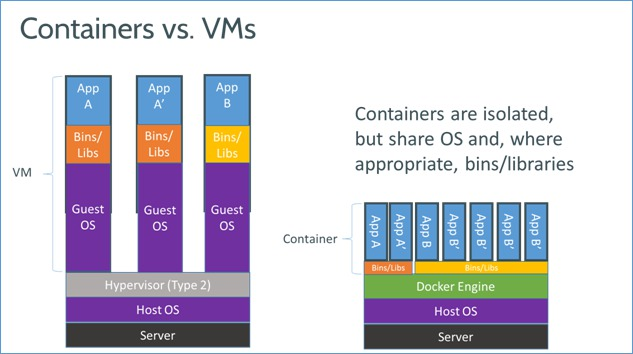
\includegraphics[scale=0.5]{img/containers_vs_vm.png}
\caption{Containers vs machines virtuelles}
\end{figure}

Les machines virtuelles possèdent leur propre OS qui embarque ses propres binaires et librairies. Ceci engendre une perte d'espace disque importante surtout si les binaires ou libraires sont communes à plusieurs machines virtuelles. De plus, démarrer une machine virtuelle prend du temps (jusqu'à plusieurs minutes). En outre, les machines virtuelles doivent installer leurs propres drivers afin de communiquer avec l'hyperviseur (logiciel s'exécutant à l'intérieur d'un OS hôte qui gère les machines virtuelles). Un avantage cependant est l'isolation complète d'une machine virtuelle qui ne peut communiquer avec les autres par défaut.

Les containers s'exécutent de manière isolée par dessus l'OS hôte qui partage ses ressources (kernel, binaires, librairies, périphériques...). Plus légers, les containers démarrent en quelques secondes seulement. Sur une machine, il est tout à fait possible de lancer de milliers de containers similaires, car l'empreinte mémoire est réduite et l'espace disque occupé est partagé si les containers sont semblables. Ceci est expliqué plus en détail à la section \ref{pres-docker-systeme-fichiers-couches}. Les containers sont isolés, mais ils peuvent aussi communiquer entre eux si on leur a explicitement donné l'autorisation.

Si le lecteur désire connaître plus de détails concernant la virtualisation, il est conseillé de lire le chapitre 3.2 du rapport "\bassangPrjSemestre" de M. Loic Bassang \cite{bassang_semestre} qui amène une bonne introduction aux différents types de virtualisation.


\section{Docker images et Docker containers}
Avec Docker, une application est encapsulée avec toutes ses dépendances et sa configuration dans une \textbf{image}. 

Pour construire cette image, on utilise un Dockerfile. Il s'agit d'un fichier qui décrit les étapes de création et de configuration nécessaires à l'obtention de l'application configurée. C'est dans ce fichier qu'on retrouve l'OS à utiliser, les dépendances à installer et toutes autres configurations utiles au bon fonctionnement de l'application à déployer. 

Typiquement un Dockerfile permettant de lancer un serveur web Nginx qui affiche un "hello world" ressemble à ceci :

\begin{bashcode}
FROM alpine  # image de départ
MAINTAINER support@tutum.co  # mainteneur du Dockerfile
RUN apk --update add nginx php-fpm && \  # installation des dépendances
    mkdir -p /var/log/nginx && \
    touch /var/log/nginx/access.log && \
    mkdir -p /tmp/nginx && \
    echo "clear_env = no" >> /etc/php/php-fpm.conf
ADD www /www  # ajout des sources de l'application
ADD nginx.conf /etc/nginx/  # ajout d'un fichier de configuration
EXPOSE 80  # ouverture du port 80
CMD php-fpm -d variables_order="EGPCS" && (tail -F /var/log/nginx/access.log &) && exec nginx -g "daemon off;" # commande à lancer au lancement du container
\end{bashcode}

Source: \url{https://github.com/tutumcloud/hello-world/blob/master/Dockerfile}

Un Dockerfile est en quelque sorte la recette de cuisine qui permet de construire une image Docker.

Une fois l'image construite, on peut exécuter l'application dans un container. Un container Docker est donc une instance de l'image fraîchement créée. La figure \ref{docker-dockerfile-image-container} montre les relations entre un Dockerfile, une image et un container.

\begin{figure}[hbtp]
\centering
\includegraphics[scale=0.7]{img/docker-dockerfile-image-container.png}
\caption{Dockerfile, image et container}
\label{docker-dockerfile-image-container}
\end{figure}


\section{Système de fichiers en couche}\label{pres-docker-systeme-fichiers-couches}
Chaque image Docker est composée d'une liste de couches (\textit{layers}) superposées en lecture seule\cite{understanding_image_container_driver_storage}. Chaque couche représente la différence du système de fichiers par rapport à la couche précédente. Sur la figure \ref{docker-image-layers}, on peut voir 4 couches (identifiables avec des ID) et leur taille respective.

\begin{figure}[hbtp]
\centering
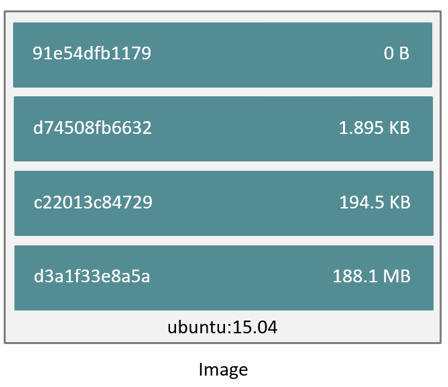
\includegraphics[scale=0.8]{img/image-layers}
\caption{Couches d'une image Docker}
\label{docker-image-layers}
\end{figure}

À la création d'un container, une nouvelle couche fine est ajoutée. Cette couche, appelée "container layer" est accessible en écriture durant l'exécution du container. La figure \ref{docker-container-layers} le montre clairement.

\begin{figure}[hbtp]
\centering
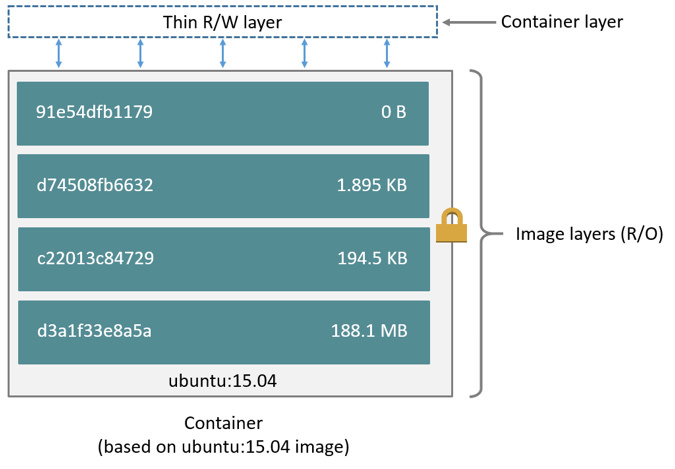
\includegraphics[scale=0.8]{img/container-layers}
\caption{Couches d'un container Docker}
\label{docker-container-layers}
\end{figure}

Un mot supplémentaire sur une nouvelle caractéristique arrivée avec Docker 1.10 (mars 2016); avant cette version, Docker attribuait des UUID\footnote{UUID : \url{https://fr.wikipedia.org/wiki/Universal_Unique_Identifier}} générés aléatoirement pour identifier les couches d'une image. Désormais, ces UUID sont remplacés par des hash appelés \textit{secure content hash}.

Les différences principales entre un UUID et un hash sont :
\begin{itemize}
\item Un UUID est généré aléatoirement, donc deux images exactement identiques auront un UUID différent alors qu'en utilisant un hash, le résultat sera identique
\item Avec les UUID, même si la probabilité est rare\footnote{Probabilité de doublon : \url{https://en.wikipedia.org/wiki/Universally_unique_identifier\#Random_UUID_probability_of_duplicates}}, il est possible de générer deux fois le même UUID ce qui peut poser des problèmes lors de la construction des images
\item Une image téléchargée chez une personne A aura un UUID différent que la même image téléchargée chez une personne B. Impossible de s'assurer de l'intégrité de l'image téléchargée en se basant sur l'UUID. En utilisant le hash, on s'assure du même résultat si l'image est identique
\end{itemize}

\vspace{2mm}
Par conséquent, Docker avance les avantages suivants:
\begin{itemize}
\item Intégrité des images téléchargées et envoyées (sur Docker Hub par exemple)
\item Évite les collisions lors de l'identification des images et des couches
\item Permet de partager des couches identiques qui proviendraient de \textit{build} différents
\end{itemize}

Le dernier point est relativement intéressant. En effet, si deux images de base (Ubuntu et Debian) sont différentes, mais qu'une couche supérieure est identique (par exemple l'ajout d'un même fichier texte) alors cette couche supérieure peut être partagée entre les deux images (puisqu'elle possède le même hash). Ceci peut potentiellement offrir un gain d'espace disque conséquent si plusieurs images partagent plusieurs couches identiques. Ceci n'aurait pas pu être possible avec les UUID, car les deux couches auraient produit deux UUID différents. Un exemple est visible à la figure \ref{shared-layer-hash}

\begin{figure}[hbtp]
\centering
\includegraphics[scale=0.7]{img/shared-layer-hash}
\caption{Couche partagée entre deux images Docker}
\label{shared-layer-hash}
\end{figure}

D'autres explications plus détaillées sur le système de fichiers en couches ont fait l'objet du chapitre 5.4.1 du rapport "\bassangPrjSemestre" de M. Loic Bassang.


\section{Isolation}\label{pres-docker-isolation}
Docker met en avant le fait que ses containers soient isolés du système hôte. Pour ce faire, Docker utilise des mécanismes fournis par le kernel. On peut citer parmi ces mécanismes les \textit{namespaces} et \textit{cgroups}.

\subsection{Les namespaces}
Les namespaces permettent d'isoler certaines fonctionnalités d'un système d'exploitation utilisant Linux. Comme chroot permet aux processus de voir comme racine un dossier isolé du système et non pas la "vraie" racine, les namespaces isolent certains aspects du système comme les processus, les interfaces réseaux, les points de montage, etc.

Jusqu'à très récemment (docker < 1.10.0), Docker supportait les namespaces suivants\cite{docker_1_10_user_namespace}:

\begin{itemize}
\item PID namespace, chaque conteneur a ses propres id de processus
\item UTS namespace, pour avoir son propre hostname
\item IPC namespace, qui permet d'isoler les Communications Inter-Processus
\item Network namespace, chaque conteneur peut avoir sa propre interface réseau, son IP, ses règles de filtrage
\end{itemize}

Docker a désormais ajouté le support d'un nouveau namespace: user namespace. Celui-ci permet à un processus d'avoir les droits root au sein d'un namespace, mais pas en dehors. Avant, Docker lançait les containers en root ce qui pouvait poser des problèmes de sécurité si un processus dans le container venait à en sortir; il se retrouverait root sur le système hôte. Avec la prise en charge de ce namespace, un container Docker a l'impression d'être root alors qu'il n'est, en réalité, qu'un utilisateur normal sur le système hôte.

\subsection{cgroups - Control Groups}
Cgroups (control groups) est une fonctionnalité du kernel pour limiter, prioriser, isoler et contrôler l'utilisation des ressources (CPU, RAM, utilisation disque, utilisation réseau...). Pour limiter les ressources, cgroups propose de créer un groupe (profil) qui décrit les limitations à respecter. Par exemple, Si on crée un groupe appelé "groupe 1" et qu'on exige de lui qu'il n'utilise qu'au maximum 25\% de la charge CPU et n'utilise qu'au maximum 100 MB de RAM. Alors, il devient possible de lancer des programmes qui appartiennent à ce groupe et qui respectent les limites fixées.

Lorsqu'on utilise la commande \code{docker run} de Docker pour lancer un container, Docker peut utiliser cgroups et ainsi limiter les ressources du container\footnote{Docker - Runtime constraints on resources: \url{https://docs.docker.com/engine/reference/run/\#runtime-constraints-on-resources}}.

\section{Contraintes liées au monde de l'embarqué}
On entend par système embarqué, un système qui est/peut être léger, autonome, à puissance limitée, à stockage réduit, avec un OS minimal et souvent connecté.

Dans le monde de l'embarqué, il existe plusieurs problèmes récurrents lorsqu'on développe, déploie et maintient une application sur une cible. On peut citer les problèmes suivants :

\begin{itemize}
\item Cross-compilation souvent obligatoire
\item Aucune interface graphique
\item Installation et configuration des dépendances sur la cible
\item Mises à jour de l'application et de ses dépendances
\item Tests et journalisation (logs)
\item Limiter l'utilisation en CPU, RAM et disque
\end{itemize}

Bien que ces problèmes peuvent être aussi présents dans le cas d'un développement desktop, ils ne sont pas aussi préoccupants.

Docker peut être utile dans le cadre d'une application embarquée, car il permet une maintenance plus aisée de l'application, car on peut \textbf{versionner son installation et sa configuration ainsi que celle de ses dépendances}. Ceci permet de plus facilement mettre à jour une application, mais également de pouvoir revenir à une version précédente. De plus, si un accès réseau est disponible, il est même possible d'administrer Docker à distance depuis un poste de développement en se connectant au \textit{deamon} Docker de la cible.

Cependant, il reste quelques freins et prérequis pour pouvoir utiliser Docker sur une carte embarquée :

\textbf{GNU/Linux : } Il faut un système GNU/Linux et si possible une distribution qui intègre Docker dans ses packages

\textbf{Images compatibles : } Les images doivent être compatibles avec la plateforme de la cible. Les images x64 ne fonctionnent pas sur ARM. Actuellement, la majorité des images sont basées sur une image de base x64. Dans la plupart des cas, il suffit de trouver l'équivalent ARM de l'image de base. Par exemple, à la lecture d'un Dockerfile, il suffit de remplacer \code{FROM ubuntu} par \code{FROM armhf/ubuntu} pour que l'image arrive à se construire. Dans les autres cas, il faudra adapter les instructions du Dockerfile.

\textbf{Espace disque limité : } Il faut veiller à l'utilisation de l'espace disque. En effet, la plupart des images se basent sur des Ubuntu (~400 MB) ou des Debian (~300 MB) ce qui peut être trop volumineux pour un système embarqué. De plus plusieurs versions de ces images peuvent être téléchargées si les Dockerfiles le spécifient. Par exemple, \code{FROM ubuntu:14.04} pour l'image 1 et \code{FROM ubuntu:15.10} pour l'image 2. On favorisera l'utilisation d'une image de base légère, comme Alpine Linux\footnote{Alpine Linux : \url{http://www.alpinelinux.org/}}, commune à plusieurs applications ou processus tournant sur la cible. 


\chapter{Matériel utilisé et mise en place de la cible}

Ce chapitre présente le matériel utilisé dans le projet ainsi que son installation et sa configuration de base.

Afin de réaliser ce projet, une carte embarquée \odroid a été mise à disposition afin d'y faire tourner Docker. 

\section{La carte \odroid}

Cette carte possède les caractéristiques suivantes \cite{TODO}: 

\begin{itemize}
\item Samsung Exynos5422 Cortex™-A15 1.8Ghz quad core and Cortex™-A7 quad core CPUs 
\item Mali-T628 MP6(OpenGL ES 3.0/2.0/1.1 and OpenCL 1.1 Full profile)
\item 2Gbyte LPDDR3 RAM at 933MHz (14.9GB/s memory bandwidth) PoP stacked
\item eMMC5.0 HS400 Flash Storage
\item USB 3.0 Host x 1, USB 3.0 OTG x 1, USB 2.0 Host x 4
\item HDMI 1.4a for display
\end{itemize}

\begin{figure}[hbtp]
\centering
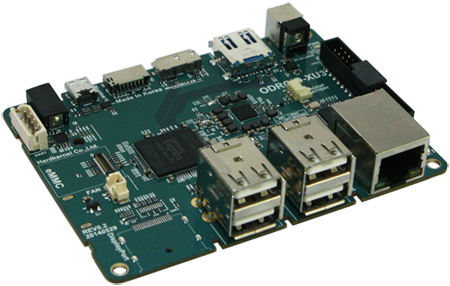
\includegraphics[scale=0.5]{img/ODROIDXU3Lite.jpg}
\caption{\odroid}
\end{figure}

\section{Installation}

Initialement, il était prévu de générer un système d'exploitation minimal qui aurait été capable de faire tourner Docker et des containers. Malheureusement, il n'a pas été possible de cross compiler Docker \textit{et son daemon} afin de lancer des containers sur ce système minimal. Plus d'informations sont disponibles dans le rapport \oldreportname. 

Ainsi, il a été décidé, de la même manière que pour le travail de bachelor précédent, d'utiliser une distribution GNU/Linux proposant Docker dans ses packages. Le choix s'est donc porté sur \textbf{Archlinux ARM} \cite{TODO}.

Sur la page wiki de la distribution (\url{https://archlinuxarm.org/platforms/armv7/samsung/odroid-xu3}), on peut suivre un guide de génération de la carte SD qui contient le système d'exploitation. Ce guide est disponible à l'appendice \ref{install_alarm_odroid}.

\chapter{Objectif 3 - TODO}

\section{Situation actuelle}
TODO: rappeler les objectifs, en particulier l'objectif courant (le 3)...

TODO: dire qu'on part d'une distribution Archlinux ARM et qu'on utilise un Odroid XU3 car pas réussi à cross compiler Docker. Tout comme cela avait été fait pour le travail de Bachelor précédent.


\section{Structure de la suite du document}

Pour ce projet, il a été décidé d'étudier la question de la sécurité avec Docker avec une approche en couches. A peu à la manière du modèle OSI\footnote{Modèle OSI: \url{https://fr.wikipedia.org/wiki/Mod\%C3\%A8le_OSI}} en réseau, chaque couche représente un ensemble de fonctionnalités qui, dans le cas de ce projet, doit faire l'objet d'une évaluation de la sécurité.

L'étude de la sécurité de Docker a donc été séparée avec les couches arbitraires suivantes:

\begin{itemize}

\item Compilation et installation de Docker : en particulier les options  de compilation

\item \nameref{config_systeme_os_hote} : configuration du kernel, configuration des options de lancement de Docker, etc.

\item \nameref{creation_utilisation_images_docker} : Bonnes pratiques et contraintes liées au monde de l'embarqué

\item \nameref{utilisation_containers}

\end{itemize}

\textbf{Remarque : } Chacune de ces couches fait l'objet d'un chapitre dans ce rapport excepté le premier point : Compilation et installation de Docker. En effet, celui-ci n'est pas traité car, comme annoncé précédemment, la cross compilation de Docker sur un système ARM n'a pas aboutie. L'effort est alors concentré sur les autres points.


\chapter{Configuration du système d'exploitation hôte}\label{config_systeme_os_hote}

TODO TODO TODO TODO TODO TODO TODO TODO TODO 
Dans ce chapitre, on présente diverses bonnes pratiques et configurations dans le but de sécuriser Docker et/ou le système l'hébergeant.

Parmi ces techniques, on peut citer :

\begin{itemize}
\item TODOchaptertitle
\item TODO
\end{itemize}

\section{Passage en revue du benchmark de sécurité : CIS Docker 1.11.0 Benchmark}

TODO décrire ce que c'est ce bench, énumerer les points testés et en explorer un certain nombre

\subsection{Ne pas utiliser AUFS}

TODO

\subsection{User namespace}

TODO

\subsection{Interdiction de la communication réseau entre containers}

TODO

\section{Séparation des données Docker dans une partition chiffrée}

TODO

\section{TODO}

TODO

\chapter{Création et utilisation des images Docker}\label{creation_utilisation_images_docker}

TODO

\chapter{Utilisation des containers}\label{utilisation_containers}

TODO

\chapter{Déroulement du projet}

\section{Planning initial}

TODO

\section{Planning final}

TODO

\chapter{Proposition d'améliorations vis à vis du travail précédent}

TODO: passer en revue et critique positivement le travail de Bachelor précédent. Dire que ce n'est pas une critique négative mais apporter un avis supplémentaire et plus récent (Docker évoluant beaucoup)
% == Bibliography
\nocite{*} % cite all
\bibliographystyle{plain}
\bibliography{bibliography}

\begin{appendices}
\chapter{Installation de Archlinux ARM sur \odroid}\label{install_alarm_odroid}

\textbf{Remarque : }Ce guide requiert l'utilisation d'un ordinateur sous GNU/Linux.

Source : \url{https://archlinuxarm.org/platforms/armv7/samsung/odroid-xu3}

\section{Micro SD Card Creation}

Replace sdX in the following instructions with the device name for the SD card as it appears on your computer.

\begin{enumerate}

\item Zero the beginning of the SD card:

\begin{bashcode}
dd if=/dev/zero of=/dev/sdX bs=1M count=8
\end{bashcode}


\item Start fdisk to partition the SD card:

\begin{bashcode}
fdisk /dev/sdX
\end{bashcode}
 

\item At the fdisk prompt, create the new partitions:
	\begin{enumerate}[a.]
		        \item Type o. This will clear out any partitions on the drive.
		        \item Type p to list partitions. There should be no partitions left.
		        \item Type n, then p for primary, 1 for the first partition on the drive, and enter twice to accept the default starting and ending sectors.
		        \item Write the partition table and exit by typing w.
	\end{enumerate}
\item Create and mount the ext4 filesystem:

\begin{bashcode}
mkfs.ext4 /dev/sdX1
mkdir root
mount /dev/sdX1 root
\end{bashcode}


\item Download and extract the root filesystem (as root, not via sudo):

\begin{bashcode}
wget http://os.archlinuxarm.org/os/ArchLinuxARM-odroid-xu3-latest.tar.gz
bsdtar -xpf ArchLinuxARM-odroid-xu3-latest.tar.gz -C root
\end{bashcode}

\item Flash the bootloader files:

\begin{bashcode}
cd root/boot
sh sd_fusing.sh /dev/sdX
cd ../..
\end{bashcode}


\item    (Optional) Set the MAC address for the onboard ethernet controller:
    \begin{enumerate}[a.]
        \item Open the file root/boot/boot.ini with a text editor.
        \item Change the MAC address being set by the setenv macaddr command to the desired address.
        \item Save and close the file.
    \end{enumerate}

\item    Unmount the partition:

    umount root

\item    Set the boot switches on the ODROID-XU3 board to boot from SD:
    \begin{enumerate}[a.]
        \item With the board oriented so you can read the ODROID-XU3 on the silkscreen, locate the two tiny switches to the left of the ethernet jack.
        \item The first switch (left) should be in the off position, which is down.
        \item The second switch (right) should be in the on position, which is up.
    \end{enumerate}
    
\item    Insert the micro SD card into the XU3, connect ethernet, and apply 5V power.
\item    Use the serial console (with a null-modem adapter if needed) or SSH to the IP address given to the board by your router.
    \begin{itemize}
        \item Login as the default user alarm with the password alarm.
        \item The default root password is root.
    \end{itemize}

\end{enumerate}

\section{eMMC Module Creation}

\begin{enumerate}
\item    Attach the eMMC module to the micro SD adapter, and plug that into your computer.

\item    Follow the above steps to install Arch Linux ARM, and boot the board with the eMMC still attached to micro SD adapter, plugged into the SD slot in the board.

\item    Re-flash the bootloader to the protected boot area of the eMMC module:
\begin{bashcode}
cd /boot
./sd_fusing.sh /dev/mmcblk0
\end{bashcode}

\item    Power off the board:
\begin{bashcode}
poweroff
\end{bashcode}

\item    Remove the micro SD adapter, and detach the eMMC module.

\item    Set the boot switches on the ODROID-XU3 board to boot from eMMC:
    \begin{enumerate}[a.]
        \item With the board oriented so you can read the ODROID-XU3 on the silkscreen, locate the two tiny switches to the left of the ethernet jack.
        \item The first switch (left) should be in the on position, which is up.
        \item The second switch (right) should be in the on position, which is up.
    \end{enumerate}
    
\item    Connect the eMMC module to the XU3, ensuring you hear a click when doing so, connect ethernet, and apply 5V power.

\item    Use the serial console (with a null-modem adapter if needed) or SSH to the IP address given to the board by your router.
    \begin{itemize}
        \item Login as the default user alarm with the password alarm.
        \item The default root password is root.
    \end{itemize}

\end{enumerate}

\end{appendices}

\end{document}
